\documentclass{article}

% set font encoding for PDFLaTeX, XeLaTeX, or LuaTeX
\usepackage{ifxetex,ifluatex}
\if\ifxetex T\else\ifluatex T\else F\fi\fi T%
  \usepackage{fontspec}
\else
  \usepackage[T1]{fontenc}
  \usepackage[utf8]{inputenc}
  \usepackage{lmodern}
\fi

\usepackage{hyperref}

\usepackage{amsmath}
\usepackage{comment}
\usepackage{color}
\usepackage{graphicx}
\usepackage{amsfonts}
\usepackage{movie15}


\setlength{\parindent}{0pt}




\title{Title of Document}
\author{Name of Author}

% Enable SageTeX to run SageMath code right inside this LaTeX file.
% http://doc.sagemath.org/html/en/tutorial/sagetex.html
% \usepackage{sagetex}

% Enable PythonTeX to run Python – https://ctan.org/pkg/pythontex
% \usepackage{pythontex}


\begin{document}
\maketitle

\section{notas}

capa densa
capa oculta
ap. supervisado
clasificacion



crear red python keras: https://youtu.be/aFZEvQDTSyA?t=616

perceptron: unica neurona cuyo input es un vector binario y output es un numero binario. su funcion de activacion es la step function
\url{https://es.wikipedia.org/wiki/Perceptr%C3%B3n}
\url{https://wikimedia.org/api/rest_v1/media/math/render/svg/50f2b5077f8fa933c912c6ca0571d6c7d3709d83}

umbral o sesgo o threshold

perceptron multicapa 
funcion de activacion

\section{Redes Neuronales}
%Intuitivamente una red neuronal artificial es un conjunto de unidades que se conocen como neuronas (o nodos) conectadas entre sí. Las redes neuronales artificiales reciben este nombre debido a la semejanza que hay entre su representación gráfica y una red neuronal de un cerebro biológico.\\

%También es un tema de marketing por el tema de "inteligencia artificial"

Formalmente una red neuronal es un modelo matemático. El deeplearning (o también conocido como aprendizaje profundo) es la rama específica del aprendizaje automático (o machine learning) que usa redes neuronales.\\


\subsection{Perceptrón}

Un perceptrón (o neurona) es un modelo de deeplearning que recibe como input variables binarias $x_1,\hdots,x_n $ y tiene como output una única variable binaria $y$. A su vez, esta función depende de los parámetros reales $\omega_1,\hdots,\omega_n,u $. A los parámetros $\omega_i$ se les conoce como pesos y al parámetro $u$ se le conoce como umbral (o sesgo o threshold o bias)\footnote{\url{http://neuralnetworksanddeeplearning.com/chap1.html}}.\\

El perceptrón está definido por la siguiente función
$$y=\begin{cases}
0, & \text{si } \sum_{i=1}^nw_ix_i-u\leq 0\\
1, & \text{si } \sum_{i=1}^nw_ix_i-u>0
\end{cases}$$

El perceptrón sirve como modelo para tomar de decisiones basado en otros hechos. Por ejemplo, puede modelizar la siguiente toma de decisiones. Consideremos el siguiente escenario\footnote{\url{https://youtu.be/CU24iC3grq8?t=236}}:

\begin{itemize}
\item $y=$Irnos de viaje
\item $x_1=$Tengo suficiente dinero?
\item $x_2=$Mi pareja quiere ir?
\item $x_3=$Hará buen tiempo?
\end{itemize}

\textcolor{red}{Introducir grafico}\\

El perceptrón modela una posible toma de decisiones a la hora de decidir si irnos de viaje o no y de él se puede sacar su tabla de la verdad.\\

Sin embargo, un perceptrón no es capaz de modelizar cualquier toma de decisión (tabla de la verdad). Por ejemplo no es capaz de modelizar la operación lógica XOR.\\


Nótese que si fijamos $w_1,\hdots,w_n,u\in\mathbb{R} $, entonces
$$H:=\left\{x=(x_1,\hdots,x_n)\in\mathbb{R}^n \ \middle| \ y(x)=\sum_{i=1}^nw_ix_i-u= 0\right\} $$
define un hiperplano de $\mathbb{R}^n$. Desde un punto de vista geométrico, este hiperplano es el separador entre $\{x\in\{0,1\}^n \ | \ y(x)<0\} $ y $\{x\in\{0,1\}^n \ | \ y(x)>0\} $. Es decir, que el perceptrón únicamente puede hacer una separación lineal (o afín) del conjunto de puntos $\{0,1\}^n $.\\

En particular, un perceptrón no puede reproducir la operación lógica XOR.
\begin{figure}[htbp]
\centering
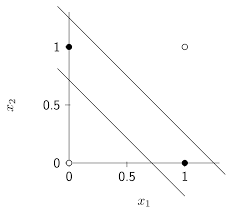
\includegraphics[width=4cm]{imagenes/XOR.png}
\caption{Visualizacación de la separación no lineal de la puerta XOR}
%foto sacada de este enlace 
% https://encrypted-tbn0.gstatic.com/images?q=tbn%3AANd9GcReKA3PNHEG6uEIRj97rpD1UHESUsqq2OzXvIzWzt7K-YSf7WPv&usqp=CAU
\end{figure}

% https://www.youtube.com/watch?v=y7NdSrkrwqI
% http://neuralnetworksanddeeplearning.com/chap1.html

\begin{figure}[htbp]
\centering
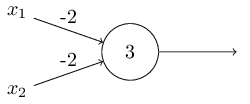
\includegraphics[width=4cm]{imagenes/NAND.png}
\caption{Perceptron modelizando una puerta NAND}
\label{fig:red_nand}
\end{figure}
En la figura \ref{fig:red_nand} se muestra una representación gráfica de un perceptrón que reproduce una puerta lógica NAND.
Esta es una red con dos capas: la primera contiene dos neuronas y la segunda solo una con un umbral igual a $3$. Además observamos que los pesos de las dos únicas conexiones son iguales a $-2$. En este caso la función de activación de la neurona de la segunda capa es 
$$f(x)=\begin{cases}
1 \text{ si } x>0\\
0 \text{ si } x\leq 0\\
\end{cases}.$$

En efecto, como se puede ver en la figura \ref{fig:tabla_verdad}, la red reproduce la tabla de la verdad de la puerta lógica NAND.\\
\begin{figure}[htbp]
\centering
\begin{tabular}{ |c|c|c| } 
 $x_1$ & $x_2$ & output \\ 
 \hline
 0 & 0 & $f(0\cdot (-2)+0\cdot (-2)+3)=f(3)=1$ \\ 
 0 & 1 & $f(0\cdot (-2)+1\cdot (-2)+3)=f(1)=1$ \\ 
 1 & 0 & $f(1\cdot (-2)+0\cdot (-2)+3)=f(1)=1$ \\ 
 1 & 1 & $f(1\cdot (-2)+1\cdot (-2)+3)=f(-1)=0$ 
\end{tabular}
\caption{Tabla de la verdad del perceptrón representado en la figura \ref{fig:red_nand}}
\label{fig:tabla_verdad}
\end{figure}



\subsection{Perceptrón multicapa}
Las puertas NAND son universales para la computación, es decir, se puede conseguir cualquier puerta lógica como combinaciones de estas\footnote{\url{http://neuralnetworksanddeeplearning.com/chap1.html}}.

\section{Redes neuronales convolucionales}

Usar una red neuronal para reconocer dígitos escritos a mano es posible pero no es lo mejor. La red recibiría los píxeles como un vector, perdiendo así la información sobre la posición relativa de los píxles de la imagen. Es natural pensar que esta información es vital para un correcto reconocimiento.\\

La red, con tal de "detectar ejes o lineas", debería aprender por sí sola que relación hay entre los inputs (intensidad de los pixeles) que esta recibe.\\

Otro aspecto a mejorar es la invarianza por traslación\footnote{\url{https://www.youtube.com/watch?v=dAetIuYz46g}}. Una red entrenada para reconocer números centrados en la imagen no sería capaz de reconocerlos si estos están a un lado de la imagen (no es capaz de generalizaar las formas y depende masivamente de la posición).

\subsection{Convolución}

\subsubsection{Filtros}
Un kernel es una matriz cuadrada $K$ con coeficientes reales. Los kernels tienen una dimensión impar, de modo que se puede hablar de su elemento principal o (central)\footnote{\url{https://datascience.stackexchange.com/questions/23183/why-convolutions-always-use-odd-numbers-as-filter-size}}.\\

Un filtro es un tensor de más de una dimensión cuyas "capas" son kernels\footnote{\url{https://stats.stackexchange.com/questions/154798/difference-between-kernel-and-filter-in-cnn}}. Es posible que un filtro contenga un único kernel, de modo que a veces estas palabras se usan indistintamente.\\

Hay distintos filtros destacables, por ejemplo:
\begin{itemize}
\item Filtro de desenfoque (o blur) 3x3: $\begin{pmatrix}
\frac{1}{9} & \frac{1}{9} & \frac{1}{9}\\
\frac{1}{9} & \frac{1}{9} & \frac{1}{9}\\
\frac{1}{9} & \frac{1}{9} & \frac{1}{9}
\end{pmatrix}$

\item Filtro vertical 3x3: $\begin{pmatrix}
-1 & 0 & 1\\
-1 & 0 & 1\\
-1 & 0 & 1
\end{pmatrix}$

\item Filtro horizontal 3x3: $\begin{pmatrix}
1 & 1 & 1\\
0 & 0 & 0\\
-1 & -1 & -1
\end{pmatrix}$

\item Edge detector 3x3: $\begin{pmatrix}
0 & -1 & 0\\
-1 & 4 & -1\\
0 & -1 & 0
\end{pmatrix}$


\end{itemize}


%\textcolor{red}{Nota: Los filtros suelen ser únicamente de dimension impar. Esto se debe a que de este modo siempre hay un píxel central en el kernel y así podemos saber a qué pixel del mapa de características corresponde. Dicho de otra manera, el kernel tiene que tener un pixel central del cual "se extraen sus características".\footnote{\url{https://datascience.stackexchange.com/questions/23183/why-convolutions-always-use-odd-numbers-as-filter-size}}}

\subsubsection{Padding}
Dada una imagen $I$ con $c$ canales de resolución $n\times n$ y una cantidad entera $p$, se conoce como hacer padding (o rellenar) con ceros a la imagen $I$ a la operación cuyo output es la nueva imagen, que denotaremos con $Pad(I,p)$, compuesta por $c$ canales de dimensión $n+2p\times n+2p$ definida como

$$Pad(I,p)[i,j,k]:=\begin{cases}
  I[i-p,j-p,k] & p\leq i,j<n+p\\
  0 & \text{En caso contrario}
\end{cases} $$


\subsubsection{Operación de convolución/correlación}

Nota: A continuación se va a definir la operación de correlación. En el ámbito de redes neuronales, se le suele llamar convolución. Esto se debe a que la única diferencia entre una correlación y una convolución es un flip de una de las entradas y en el caso de las redes, la red aprenderia a clasificar bien con los pesos "flipeados"\footnote{\url{https://youtu.be/cUa3Jug3TiA?list=PLWzLQn_hxe6ZlC9-YMt3nN0Eo-ZpOJuXd&t=590}}.

Sea $I$ una imagen con $c$ canales de resolución $n\times n$ y sea $F$ un filtro formado por $c$ kernels de dimensión $m\times m$ con $m<n$. Sean $p,s\in \mathbb{N}$. La operación de convolución de $I$ y $F$ con un stride $s$ y padding $p$ es una imagen $Conv(I,F,p,s)$ con un único canal (o feature map) de dimensión, digamos, $o\times o$.\\


% Sean $i$ y $j$ tales que 
% $$\frac{m-1}{2}\leq i,j<n-\frac{m-1}{2}. $$
El elemento $i,j$ de $Conv(I,F,p,s)$ viene definido\footnote{Inspirado en \url{https://ichi.pro/es/matematicas-de-las-redes-neuronales-convolucionales-30697178023872} \text{y a su vez traducido de} \url{https://towardsdatascience.com/convolutional-neural-networks-mathematics-1beb3e6447c0}} por

% $$I'[i,j]=\sum_{\alpha=1}^c \sum_{\beta=-\frac{m-1}{2}}^{\frac{m-1}{2}}\sum_{\gamma=-\frac{m-1}{2}}^{\frac{m-1}{2}} I[i+\beta,j+\gamma,k]\cdot F\left[\alpha+\frac{m-1}{2},\beta+\frac{m-1}{2}\right]  $$

$$Conv(I,F,p,s)[i,j]:=\sum_{\alpha=0}^c \sum_{\beta=0}^m \sum_{\gamma=0}^m Pad(I,p)[i\cdot s+\beta,j\cdot s+\gamma,\alpha]\cdot  F[\beta,\gamma,\alpha]$$

donde 
$$0\leq i\cdot s+\beta <n+2p \quad \forall i,\beta $$
y
$$0\leq j\cdot s+\gamma <n+2p \quad \forall j,\gamma .$$
Por lo tanto tenemos que  
$$o=\left\lfloor \frac{n+2p-m}{s}\right\rfloor+1$$

Nótese que si $n+2p-m$ no es múltiplo de $s$, entonces habrán filas y columnas de la imagen que se saltarán. Además, los píxeles de las esquinas y bordes tienen menor importancia en el cálculo. Este es el motivo por el cual se introduce el padding: Añadir filas y columnas redundates para que al convolución se haga con todos los píxeles de la imagen por igual.\\

Nota: Los frameworks tensorflow y keras admiten como padding la opción 'same' que quiere decir que se ajustará el padding adecuado para que tras la convolución no se pierda tamaño\footnote{\url{https://youtu.be/l16RxAmP9QE?list=PLdxQ7SoCLQANQ9fQcJ0wnnTzkFsJHlWEj&t=1376}}

\subsubsection{visualización de la operación de convolución}

Haz click \href{https://miro.medium.com/max/1052/1*GcI7G-JLAQiEoCON7xFbhg.gif}{aquí}, \href{https://cdn-media-1.freecodecamp.org/images/gb08-2i83P5wPzs3SL-vosNb6Iur5kb5ZH43}{aquí} o \href{https://thumbs.gfycat.com/AffectionateMemorableGreyhounddog-size_restricted.gif}{aquí} para ver animaciones de esta operación\footnote{fuente de los gifs: \url{https://juansensio.com/blog/042_cnns}}.

\textcolor{red}{una alternativa seria pasar a markdown para ver }\\

% A grosso modo, la convolución genera una nueva matriz conocida como feature map o mapa de características mediante productos escalares de $F$ y submatrices de $M$.\\

% Inicialmente se le hace un padding (rodear con ceros) la imagen $M$ con un número $p$ de lineas. De este modo, $M$ pasa de tener dimensiones $n\times n$ a $(n+2p)\times (n+2p) $ (se añade una fila/columna por todos los lados).\\

% A continuación se fija el stride $s$, es decir, la cantidad de píxeles que se desplazará horizontalmente el filtro. Finalmente se genera una nueva matriz $M'$ donde sus entradas son producntos componente a componente del filtro F y submatrices de $M$.\\

% En particular la $M'$ tendrá dimensiones $o\times o$ donde
% $$o=\left\lfloor \frac{n+2p-m}{s}\right\rfloor+1$$

\subsubsection{interpretación de la convolución}


\subsubsection{Estructura de la capa de convolución}

NOTA: si la imagen fuera a color, el kernel realmente sería de $3x3x3$ es decir: un filtro con 3 kernels de $3\times3$; luego  esos 3 filtros se suman (y se le suma una unidad bias) y conformarán 1 salida (cómo si fuera 1 solo canal)\footnote{\url{https://www.aprendemachinelearning.com/como-funcionan-las-convolutional-neural-networks-vision-por-ordenador/}}.\\

En realidad, no aplicaremos un solo kernel. Por ejemplo, en esta primera convolución podríamos tener 32 kernels, con lo cual realmente obtendremos 32 matrices de salida con dimensión 28x28x1, dando un total del 25.088 neuronas para nuestra PRIMER CAPA OCULTA de neuronas. Parecen muchas neuronas para una imagen cuadrada de apenas 28 pixeles. El número aumentaría drásticamente si tomáramos una imagen de entrada de 224x224x3 (que aún es considerado un tamaño pequeño)\footnote{\url{https://www.aprendemachinelearning.com/como-funcionan-las-convolutional-neural-networks-vision-por-ordenador/}}.\\

Cuando tratamos con imágenes con más de un canal (por ejemplo rgb), los filtros deben tener el  mismo número de canales (kernels?). De modo que cada kernel  hace una convolución con su canal correspondiente. Posteriormente se cogen todas esos outputs y se hace la media. De este modo, tras convolucionar el filtro con la imagen de más de un canal, se sigue teniendo una imagen con un único canal como output. En consecuencia, la cantidad de imagenes de output será igual a la cantidad de filtros que tenga esa capa convolusional. Finalmente a cada una de estas imágenes se les suma un cierto humbral y se aplica la ReLU.\footnote{\url{https://www.youtube.com/watch?v=HEH1clGg8o8&list=PLdxQ7SoCLQANQ9fQcJ0wnnTzkFsJHlWEj&index=50}}\\

Nota: por lo que veo en la libreria de tensorflow, cada kernel del filtro tiene su propio bias. tras aplicar el bias se hace la media.\footnote{\url{https://www.youtube.com/watch?v=S5MwKyYYLSM&list=PLdxQ7SoCLQANQ9fQcJ0wnnTzkFsJHlWEj&index=51}}

Nota: Por lo general se suele escoger que la cantidad de filtros sea una potencia de 2 por algún tipo de cuestión de eficiencia\footnote{\url{https://youtu.be/XkqgTaWle0I?list=PLWzLQn_hxe6ZlC9-YMt3nN0Eo-ZpOJuXd&t=61}}

\subsection{Implementación}
Una de las redes más sencillas es la LeNET-5\footnote{\url{https://www.youtube.com/watch?v=HEH1clGg8o8&list=PLdxQ7SoCLQANQ9fQcJ0wnnTzkFsJHlWEj&index=50}}\footnote{\url{https://en.wikipedia.org/wiki/LeNet}}\\

sensio -arquitecturas de cnns famosas: \url{https://www.youtube.com/watch?v=IKB8rzGU8Wo}

\section{enlaces de interes}
\begin{itemize}
\item \url{https://indoml.com/2018/03/07/student-notes-convolutional-neural-networks-cnn-introduction/} - ilustraciones muy chulas y utiles

\item webs para ayudar a redactar la seccion:
\begin{itemize}
\item \url{https://www.aprendemachinelearning.com/como-funcionan-las-convolutional-neural-networks-vision-por-ordenador/}
\item \url{https://www.youtube.com/playlist?list=PLv8Cp2NvcY8DpVcsmOT71kymgMmcr59Mf} - lista de reproduccion de un canal que habla sobre las arquitecturas de deres conocidas
\item \url{https://bootcampai.medium.com/redes-neuronales-convolucionales-5e0ce960caf8}
\end{itemize}
\item \url{https://www.youtube.com/watch?v=V8j1oENVz00} - dotcsv (HECHO)
\item \url{https://www.youtube.com/watch?v=ysqpl6w6Wzg} - dotcsv (VISTO, TODO) (interesante pero no creo que sea necesario meterlo aqui). El video empieza a partir del min 6:20. Hbala sobre comolos filtros detectan cada vez cosas más complejas y como intepretar cada unon delos filtros. Seria interesante reproducir eso. Toda esta visualizacióon la hace con "l microscopio de openAI": \url{https://microscope.openai.com/models}
\item \url{https://www.youtube.com/watch?v=_fDvfGxwW20} - sensio (VISTO, TODO) - interesante a partir del min 14:30 donde muestra una implementacionde una cnn usando pytorch. tambien son interesantes algunos gifs que ya he sacado de su web
\item \url{https://www.youtube.com/watch?v=AwTH_0yW9_I} - Ringa Tech (HECHO)
\item \url{https://www.youtube.com/watch?v=0zbhg79i_Bs} - indio cnn desde 0 (OPCIONAL CREO)
\item \url{https://www.youtube.com/watch?v=AwTH_0yW9_I&t=584s} - operadores importantes: operador Sobel y Algoritmo de Canny (OPCIONAL)
\item \url{https://stackoverflow.com/questions/67409505/python-2d-convolution-optimization} - curiosa implementacion en python de una visualizacion ascii de la convolucion
\item \url{https://www.youtube.com/watch?v=OYXkoZXEZc4&list=PLkgbkukKg_Nr-CAmU1yGbhJ8UELVDJ07I} - sensio (FALTA) - lista de reproduccion en la que parece que implementa unlocalizador de objetos y segmentador de imagenes desde cero. seguramente lo hagaa partir de torch pero no esta mal
\end{itemize}



\subsection{Max-Pooling (deberia ser poolig en general porque tambien hay average pooling)}
Si hiciéramos una nueva convolución a partir de esta capa, el número de neuronas de la próxima capa se iría por las nubes (y ello implica mayor procesamiento)! Para reducir el tamaño de la próxima capa de neuronas haremos un proceso de subsampling en el que reduciremos el tamaño de nuestras imágenes filtradas pero en donde deberán prevalecer las características más importantes que detectó cada filtro. Hay diversos tipos de subsampling, yo comentaré el “más usado”: Max-Pooling\footnote{\url{https://www.aprendemachinelearning.com/como-funcionan-las-convolutional-neural-networks-vision-por-ordenador/}}\\

Estas capas también aplican un filtro sobre su entrada, pero en este caso es un solo filtro que además no tiene parámetros sino que aplica una función predeterminada en su campo receptivo (mínimo, máximo (maxpooling), promedio (average pooling o avgpooling, etc)\footnote{\url{https://juansensio.com/blog/042_cnns}}.\\

Haz click \href{https://miro.medium.com/max/1456/1*WvHC5bKyrHa7Wm3ca-pXtg.gif}{aquí} para ver un gif sobre el  max-pooling.
% gif sacado de https://juansensio.com/blog/042_cnns

\section{Generalidades sobre las imágenes}

\subsection{Canales de las imágenes}
Las imágenes en blanco y negro se pueden representar con un único canal, es deicr, con una matriz de enteros en el rango $[0,255]$ o floats en el rango $[0,1]$.\\

Si la imagen es de color, entonces se representan mediante los tres canales RGB. De modo que una imagen en color se representa mediante un tensor (martriz) tridimensional.\\

En general una "imagen" podría tener tantos canales como se quisiera. Por ejemplo las redes neuronales convolucionales producen imagenes con muchos canales.

\subsubsection{Orden de los canales de las imágenes}
No hay un consenso en el orden de los indices que deben representar la altura, anchura y canales de una imagen. Por ejemplo una imagen con $c$ canales, una altura $h$ y una anchura $w$ podría representarse de las dos siguientes formas\footnote{\url{https://machinelearningmastery.com/a-gentle-introduction-to-channels-first-and-channels-last-image-formats-for-deep-learning}}.\\

\begin{enumerate}
  \item Channels First: Tensor de dimensiones $c\times h\times w$ (Como por ejemplo pytorch)
  \item Channels Last: Tensor de dimensiones $h\times w\times c$ (como por ejemplo tensorflow y numpy)
\end{enumerate}

La manera más rápida de pasar de un formato a otro (permutar los ejes) es usando numpy.transpose\footnote{\url{https://stackoverflow.com/questions/43829711/what-is-the-correct-way-to-change-image-channel-ordering-between-channels-first}}



\subsection{Input de las redes neuronales}

La arquitectura de una red neuronal podría adaptarse para tener como input una imagen con dimensiones cualesquiera.\\

Sin embargo, normalmente se deciden diseñar las redes "para uso público" y para recibir imágenes cuadradas y que cada uno haga el reshape correspondiente. No hay ninguna limitación en las posibles estructuras de las CNNs que limiten la forma del input.\footnote{\url{https://ai.stackexchange.com/questions/8323/how-to-handle-rectangular-images-in-convolutional-neural-networks}}

\section{Redes convolucionales}
En realidad la seccion deberia tener estas subsecciones aunque quizas en otro ordenador (por ejemplo la itepretacion/idea deberia ir primero)

\subsection{Capa de convolución}

\subsubsection{Filtros}

\subsubsection{padding}

\subsubsection{definicion forma/funcionamiento de la operacion de convolución}

\subsubsection{visualizacion de la convolución}
aqui deberian ir gifs y visualizacion del stride etc

\subsubsection{interpretacion de la convolucion}
filtros lineas verticales etc. estaria bien preparar un script con algun ejemplo real para ver que pasa

\subsubsection{Estructura de la capa de convolucion}

consiste de varios fltros y tienen bias y relu. 


\subsection{Capa de pooling}
hablar del max pooling o average pooling

\subsection{Estructura clásica de una cnn}

\subsection{backpropagration}
hablar de como se optmizan los filtros

\subsection{representacion grafica de una capa convolucional/redes convolucionales}
un cuadrado mas o menos gordito etc

\subsection{aruitecturas de cnns famosas}
hablarde las arquitecturas o implementar alguna


\section{Historia}

La siguiente información ha sdo obtenida de ChatGPT:\\


La arquitectura LeNet-5 fue presentada por primera vez en un artículo titulado "Gradient-Based Learning Applied to Document Recognition" publicado por Yann LeCun, Léon Bottou, Yoshua Bengio, y Patrick Haffner en 1998. En este artículo, los autores demostraron el rendimiento superior de la arquitectura LeNet-5 en la tarea de reconocimiento de dígitos escritos a mano en comparación con otras técnicas de la época. Desde entonces, la arquitectura LeNet-5 se ha utilizado como base para muchas otras arquitecturas de redes neuronales convolucionales.\\


Antes de la introducción de LeNet-5, se utilizaron varias técnicas para reconocimiento de dígitos escritos a mano, como la segmentación de imágenes, el análisis de características manuales y el uso de redes neuronales simples. En particular, el algoritmo de K-nearest neighbors (K-NN) y el algoritmo de redes neuronales de retropropagación se utilizaban comúnmente para esta tarea. Sin embargo, estos métodos no eran tan efectivos como LeNet-5 y tenían limitaciones significativas en términos de precisión y eficiencia en el entrenamiento y la inferencia.\\


La arquitectura que superó a LeNet-5 en términos de rendimiento y popularidad fue AlexNet, presentada en 2012 por Alex Krizhevsky, Ilya Sutskever y Geoffrey Hinton. AlexNet fue entrenada en un conjunto de datos mucho más grande que LeNet-5, utilizando técnicas como la regularización y el aumento de datos para reducir el sobreajuste y mejorar la precisión. AlexNet también presentó varias innovaciones, como el uso de unidades de activación no lineales ReLU, la normalización por lotes y la utilización de una GPU para acelerar el entrenamiento. Estas técnicas permitieron a AlexNet lograr una precisión sin precedentes en la tarea de clasificación de imágenes, lo que allanó el camino para el desarrollo de arquitecturas aún más grandes y sofisticadas en los años siguientes.\\


Después de AlexNet, se desarrollaron muchas arquitecturas más grandes y sofisticadas, que lograron una precisión aún mayor en tareas de visión por computadora. Entre las más importantes se encuentran:

\begin{itemize}
  \item VGG (2014): presentada por Karen Simonyan y Andrew Zisserman, esta arquitectura consta de varias capas convolucionales muy profundas y fue la primera en demostrar que el aumento del número de capas puede mejorar significativamente la precisión.
  \item Inception (2014): desarrollada por Christian Szegedy y su equipo en Google, esta arquitectura utiliza filtros de múltiples tamaños en paralelo y una estructura de bloques en cascada para mejorar la eficiencia computacional y la precisión.
  \item ResNet (2015): desarrollada por Kaiming He y su equipo en Microsoft, esta arquitectura utiliza conexiones de salto (skip connections) para permitir que la información fluya directamente a través de las capas sin ser atenuada por la función de activación, lo que permite construir redes extremadamente profundas con una precisión aún mayor.
  \item DenseNet (2016): desarrollada por Gao Huang y su equipo en el Laboratorio de IA de Google, esta arquitectura utiliza conexiones densas entre capas para permitir que cada capa reciba información de todas las capas anteriores en la red, lo que reduce el riesgo de desvanecimiento del gradiente y mejora la precisión.
  \item EfficientNet (2019): desarrollada por Mingxing Tan y Quoc V. Le en Google, esta arquitectura utiliza un enfoque de escalado compuesto para optimizar el tamaño, la profundidad y la resolución de la red para obtener la mejor relación rendimiento-eficiencia para una tarea dada.
\end{itemize}

Cada una de estas arquitecturas ha introducido innovaciones significativas y ha establecido nuevos récords de precisión en tareas de visión por computadora.\\


La primera red neuronal convolucional para detección de objetos se llamó R-CNN (Region-based Convolutional Neural Network) y fue presentada por Ross Girshick en 2014. La arquitectura de R-CNN se basa en el uso de una red neuronal convolucional para extraer características de la imagen y un clasificador SVM para clasificar cada región propuesta. R-CNN fue un gran avance en la tarea de detección de objetos y logró superar con creces los métodos tradicionales basados en características de bajo nivel y clasificadores manuales. Desde entonces, han surgido muchas otras arquitecturas para la detección de objetos, incluyendo Fast R-CNN, Faster R-CNN, YOLO (You Only Look Once) y SSD (Single Shot Detector).
\end{document}


